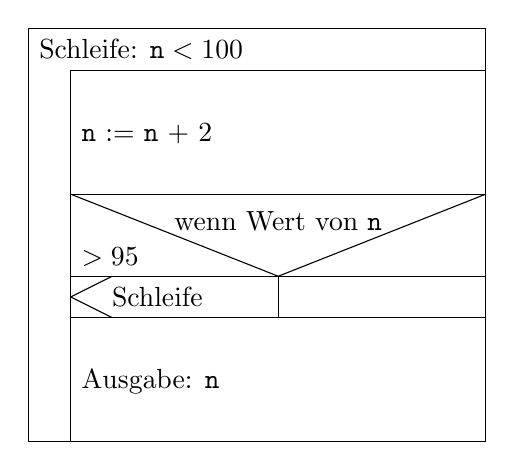
\begin{tikzpicture}
    \draw (0pt,0pt) rectangle (165.33552pt, -149.18126pt);
    \node at (4.0pt, -74.59063pt) {};
    \node at (40.79164pt, -7.6677100000000005pt) {Schleife: $\texttt{n} < 100$};
    \draw (15.33542pt,-15.33542pt) rectangle (165.33552pt, -59.950700000000005pt);
    \node at (42.918735pt, -38.05972500000001pt) {\texttt{n} := \texttt{n} + 2};
    \draw (15.33542pt,-59.950700000000005pt) rectangle (165.33552pt, -89.62154000000001pt);
    \node at (19.33542pt, -74.78612000000001pt) {};
    \draw (15.33542pt, -59.950700000000005pt) -- (90.33547pt, -89.62154000000001pt);
    \draw (90.33547pt, -89.62154000000001pt) -- (165.33552pt, -59.950700000000005pt);
    \node at (29.61319pt, -82.59481000000002pt) {$> 95$};
    \node at (161.33552pt, -85.62154000000001pt) {};
    \node at (90.33547pt, -69.84098pt) {wenn Wert von \texttt{n}};
    \draw (15.33542pt,-89.62154000000001pt) rectangle (90.33547pt, -104.56598000000002pt);
    \node at (19.33542pt, -97.09376000000002pt) {};
    \node at (46.668775pt, -97.09376pt) {Schleife};
    \draw (30.27986pt, -89.62154000000001pt) -- (15.33542pt, -97.09376000000002pt);
    \draw (15.33542pt, -97.09376000000002pt) -- (30.27986pt, -104.56598000000002pt);
    \draw (90.33547pt,-89.62154000000001pt) rectangle (165.33552pt, -104.56598000000002pt);
    \node at (94.33547pt, -97.09376000000002pt) {};
    \draw (15.33542pt,-104.56598000000001pt) rectangle (165.33552pt, -149.18126pt);
    \node at (44.210445pt, -127.84584000000001pt) {Ausgabe: \texttt{n}};
\end{tikzpicture}
